\section*{Bewegung in drei Raumrichtungen}

\subsection*{Vektoren}
Physikalische Grössen wie die Geschwindigkeit $v$, die Beschleunigung $a$ oder auch der Weg $s$ sind
vektorielle Grössen. Ein Vektor hat nicht nur eine Grösse, sondern auch noch eine Richtung.
Vektoren werden daher oft als Pfeile gezeichnet. Die Länge des Pfeils ist dann der Betrag des Vektors,
die Richtung des Pfeils gibt die Richtung des Vektors an.

Ein Vektor kann mit einem geeigneten Koordinatensystem in Komponenten zerlegt werden.


Vektoren kann man graphisch addieren.

%
\section*{Addition von Kräften}

In einem Knoten laufen drei Fäden zusammen. An dem jeweils anderen Ende der Fäden ist eine Masse angehängt.
Zwei der drei Fäden werden durch Rollen umgelenkt.
Wird der Knoten aus seiner Ruhelage (Gleichgewichtslage) ausgelenkt, so pendelt sich das System wieder in diese Lage zurück.
Die Rollen lenken die Fadenkräfte um, ändern aber nicht ihren Betrag.
In der Ruhelage ist die Summe aller angreifenden Kräfte Null.

\Einbinden{\dir/vektoren01.tex}
\Einbinden{\dir/vektoren02.tex}
\Einbinden{\dir/vektoren03.tex}
\Einbinden{\dir/vektoren04.tex}


\newpage
\section*{Zerlegung von Kräften}

Vektoren lassen sich nicht nur addieren, sondern man kann sie auch in Komponenten zerlegen. Das ist im Prinzip die Umkehrung
der Vektoraddition.

\Einbinden{\dir/vektoren05.tex}
\Einbinden{\dir/vektoren06.tex}


Ist die Richtung eines Vektors vorgegeben, lässt sich der Vektor noch nicht eindeutig zerlegen. Es gibt immer
noch viele verschiedene Möglichkeiten den Vektor zu zerlegen.

\newpage


Sind die Richtungen von zwei Vektoren gegeben (in 2D), ist die Zerlegung eindeutig möglich. Allgemein gilt, dass man
für jede Raumdimension eine eindeutige Richtung benötigt.

\Einbinden{\dir/vektoren07.tex}


In der Praxis zerlegt man Vektoren oft in Kartesische Koordinaten, also in eine $x$-, eine $y$- und im Fall von drei Dimensionen in eine $z$-Koordinate.

\Einbinden{\dir/vektoren08.tex}

\newpage

\Einbinden{\dir/vektoren09.tex}

\newpage
\Einbinden{\dir/vektoren10.tex}

\Einbinden{\dir/vektoren11.tex}


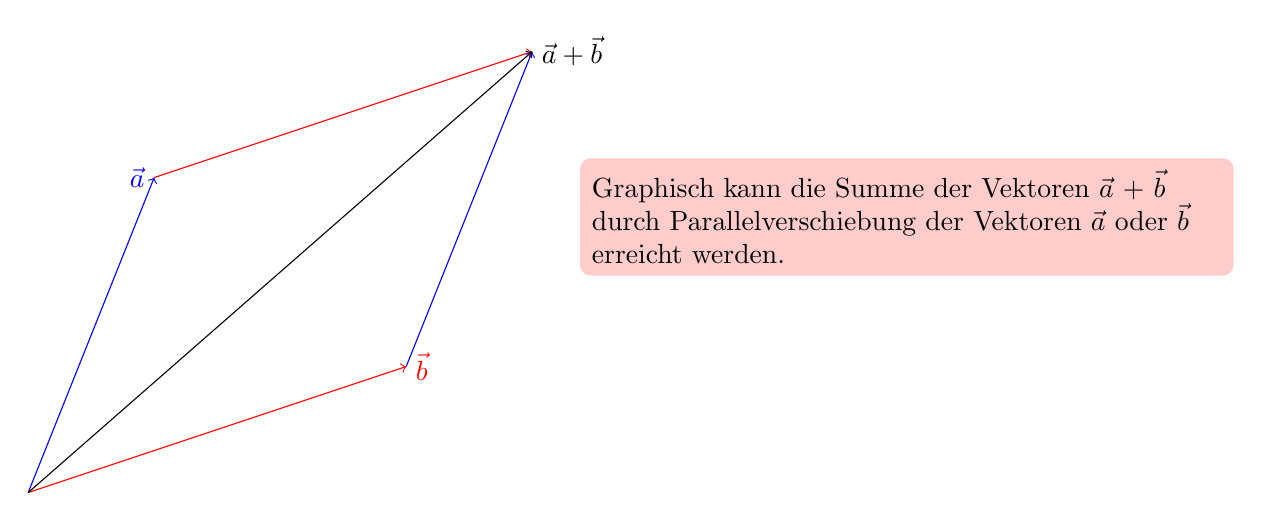
\begin{tikzpicture}[info text/.style={rounded corners, fill=red!20, inner sep=1ex}]
%\begin{tikzpicture}
%\usetikzlibrary{calc,intersections,through,backgrounds}
%\usetikzlibrary{decorations.pathmorphing}
%\draw[step=0.5cm,lightgray] (-0.5,-3.0) grid (6.5,5.0);


\draw [->, blue,scale=0.8] (0,0)--(2,5) node [left] {$\vec{a}$};
\draw[->,red,scale=0.8] (2,5)--+(6,2);

\draw[->,red,scale=0.8] (0,0)--(6,2) node [right] {$\vec{b}$};

\draw[->,blue,scale=0.8] (6,2)--+(2,5);


\draw[->,black,scale=0.8](0,0)--(8,7) node [right]{$\vec{a}+\vec{b}$};
%infokasten
\draw [xshift=7.0cm] (0,3.5) node [right, text width=8cm, info text] {
Graphisch kann die Summe der Vektoren $\vec{a}+\vec{b}$ durch Parallelverschiebung
der Vektoren $\vec{a}$ oder $\vec{b}$ erreicht werden.
};

\end{tikzpicture}

Das bedeutet, dass man eine komplizierte Bewegung, wie zum Beispiel die Bewegung eines geworfenen
Balls, oder einer Pistolenkugel für jede Raumrichtung unabhängig voneinander lösen kann.
Dies macht es erst möglich Bewegungsabläufe in mehr als einer Dimension zu berechnen.

\Einbinden{\dir/bew3d01.tex}
\Einbinden{\dir/bew3d02.tex}


